%
% 修士学位請求論文(副・正)テンプレート
% MasterThesisSample.tex
% By KASHINA, Yuki (EM-14003)
%
\documentclass{MasterThesis}
%\documentclass[fleqn]{MasterThesis} %数式を左寄せ


%%%%%%%%%%%%%%%%%%%%%%%%%%%%%%%%%%%%%%%%%%
% ユーザ任意のパッケージ
%%%%%%%%%%%%%%%%%%%%%%%%%%%%%%%%%%%%%%%%%%
%\usepackage{booktabs}
%\usepackage{multirow}
\usepackage[dvipdfmx]{xcolor}
\usepackage{otf}


%%%%%%%%%%%%%%%%%%%%%%%%%%%%%%%%%%%%%%%%%%
% マクロ
%%%%%%%%%%%%%%%%%%%%%%%%%%%%%%%%%%%%%%%%%%
%<local definition>
\newcommand{\texcmd}[1]{\texttt{\textbackslash{}#1}}

\usepackage{setspace}
\def\commentary#1{\raisebox{\baselineskip}{\parbox{0.8\textwidth}{\begin{spacing}{0.8}#1\end{spacing}}}\vspace{.42\baselineskip}\endgraf}
%</local definition>


%%%%%%%%%%%%%%%%%%%%%%%%%%%%%%%%%%%%%%%%%%
% ルートパス
%%%%%%%%%%%%%%%%%%%%%%%%%%%%%%%%%%%%%%%%%%
\graphicspath{{figure/}}
\tablepath{{table/}}


%%%%%%%%%%%%%%%%%%%%%%%%%%%%%%%%%%%%%%%%%%
% 行間調整
%%%%%%%%%%%%%%%%%%%%%%%%%%%%%%%%%%%%%%%%%%
\renewcommand{\baselinestretch}{1.0}


%%%%%%%%%%%%%%%%%%%%%%%%%%%%%%%%%%%%%%%%%%
% 図表キャプションの接頭辞
%%%%%%%%%%%%%%%%%%%%%%%%%%%%%%%%%%%%%%%%%%
%\renewcommand{\jfigurename}{図}
%\renewcommand{\jtablename}{表}
%\renewcommand{\efigurename}{Fig.~}
%\renewcommand{\etablename}{Table~}


%%%%%%%%%%%%%%%%%%%%%%%%%%%%%%%%%%%%%%%%%%
% フォントサイズ
%%%%%%%%%%%%%%%%%%%%%%%%%%%%%%%%%%%%%%%%%%
%%% 英文タイトル
%\renewcommand{\etitlefontsize}{\fontsize{21pt}{21pt}}
\renewcommand{\etitlefontsize}{\fontsize{14pt}{14pt}}

%%% 本文
%\renewcommand{\mainfontsize}{\fontsize{14pt}{25pt}}
\renewcommand{\mainfontsize}{\fontsize{12pt}{21pt}}

%%% キャプション
%\renewcommand{\captionfontsize}{\fontsize{14pt}{17pt}}
\renewcommand{\captionfontsize}{\fontsize{11pt}{14pt}}


%%%%%%%%%%%%%%%%%%%%%%%%%%%%%%%%%%%%%%%%%%
% 書誌情報
%%%%%%%%%%%%%%%%%%%%%%%%%%%%%%%%%%%%%%%%%%
%%% 和文タイトル
% \newlineで改行,数式やコマンド,クォートは{}でグルーピング
\jtitle{MasterThesisクラスの使い方{(v2.0.1)}}

%%% 英文タイトル
% \newlineで改行,数式やコマンド,クォートは{}でグルーピング
\etitle{How to use the {``}MasterThesis.cls{''} (v2.0.1)}

%%% 所属専攻 //工学研究科は不要
\affiliate{情報学専攻}

%%% 氏名・学籍番号 //\ruby{漢字}{かん|じ}, 性名間に半角空白を挿入
\author{\ruby{加科}{か|しな}~\ruby{優希}{ゆう|き}}

%%% 指導教官名・指導教官役職 //姓名間に半角空白を挿入
\supervisor{工学院~太郎}{教授}

%%% 修了年月(西暦) //全角を推奨
\ptdate{2016}{3}

%%% 前文のタイトル
\abstractname{要旨}{Abstract}

%%% 目次の有効化
\toctrue

%%% 図目次の有効化
\loftrue

%%% 表目次の有効化
\lottrue

%%% 索引の有効化
%\makeindex

%%% 研究室内部資料セクション(付録)の有効化
%\domestictrue



%%%%%%%%%%%%%%%%%%%%%%%%%%%%%%%%%%%%%%%%%%
% 書誌情報の設定終了
%%%%%%%%%%%%%%%%%%%%%%%%%%%%%%%%%%%%%%%%%%
\eom



%%%%%%%%%%%%%%%%%%%%%%%%%%%%%%%%%%%%%%%%%%
% 前文(和文)
\jabstract
%%%%%%%%%%%%%%%%%%%%%%%%%%%%%%%%%%%%%%%%%%
修士論文のフォーマットです。\LaTeX の基本的知識を有する方の利用を前提としています。以下はダミーテキストです。

情報学専攻は、情報を単に工学的な一要素として取り扱うのみでは不十分なため、文系学部卒業生も含めて情報技術について基礎的知識と興味を有する人材を積極的に受け入れる目的志向型の専攻です。情報学専攻は、基礎、工学、社会科学、これらの融合/境界領域、未踏分野の5 本柱を立て、数理的基礎理論、インターネットやモバイルに象徴されるネットワークやセキュリティ技術とその応用、ソフトウェア諸技術やコンピュータのアーキテクチャ、メディア処理技術とその技術の福祉や人間・物体の認識などへの応用、人工知能、人間工学、そして社会科学など、ハードウェアからソフトウェアまで幅広くカバーすることを目標としています。また、産官学連携については、教育的側面も含め積極的に進めています。
\footnote{``http://www.kogakuin.ac.jp/faculty/daigakuin/me/index.html''より。}



%%%%%%%%%%%%%%%%%%%%%%%%%%%%%%%%%%%%%%%%%%
% 前文(英文)
\eabstract
%%%%%%%%%%%%%%%%%%%%%%%%%%%%%%%%%%%%%%%%%%
Following text that's dummy for an English sentence.

Major of Informatics extensively covers the study from hardware to software which consists of 5 fields, basic, engineering, social sciences, and fusion of basic, engineering and social sciences/interdisciplinary field and unexplored field.We are equipped with experienced staffs and facilities to lead the fast-moving telecommunications.

In Major of Informatics, it is insufficient to consider information just as an element of engineering, therefore we are actively taking in talent having interests and fundamental knowledge in information technology, including graduates from liberal arts, to achieve objectives.Major of Informatics consists of 5 fields, which are basic, engineering, social sciences, and fusion of basic, engineering and social sciences/interdisciplinary field and unexplored field, in which you can study mathematical basic theory, network/security technology represented by internet/mobile phone and its application, software technology and computer architecture, media processing technology and application of the technology for welfare and recognition of human/object etc., artificial intelligence, human engineering, and social sciences etc.We are aiming for extensively covering study from hardware to software and aggressively working on collaboration of industry-government-academia, including educational aspects.%
\footnote{This is dummy text from ``http://www.kogakuin.ac.jp/english/graduateschool/principles/informatics-program.html''.}



%%%%%%%%%%%%%%%%%%%%%%%%%%%%%%%%%%%%%%%%%%
% 本文の開始
%%%%%%%%%%%%%%%%%%%%%%%%%%%%%%%%%%%%%%%%%%
\main



%%%%%%%%%%%%%%%%%%%%%%%%%%%%%%%%%%%%%%%%%%
% はじめに
\chapter{はじめに}
%%%%%%%%%%%%%%%%%%%%%%%%%%%%%%%%%%%%%%%%%%
この修士論文のクラスファイルとテンプレートのセットは,ある程度\LaTeX の知識がある方の利用を前提としています。そのため,章の追加等の基本的な事項は説明から省略しています。本テンプレートは\pLaTeX とdvipdfmxの組み合わせでPDFを生成する使用法を想定しています。

%\section{Windowsでの使用時に想定されるエラーへの対処}
\pLaTeX において文字コードの推定を行う設定で使用している場合,文字コードが正しく検出されないためにタイプセットが失敗する可能性があります(\fref{ts_failed})。このため,
\begin{center}
	\texttt{-kanji=utf8 -no-guess-input-enc}
\end{center}
オプションを付加し,明示的に文字コードを指定して文字コードの推定を行わないようにすることでタイプセットすることができます。%(\fref{ts_success})。

\begin{figure}[tb]
	\centering
	%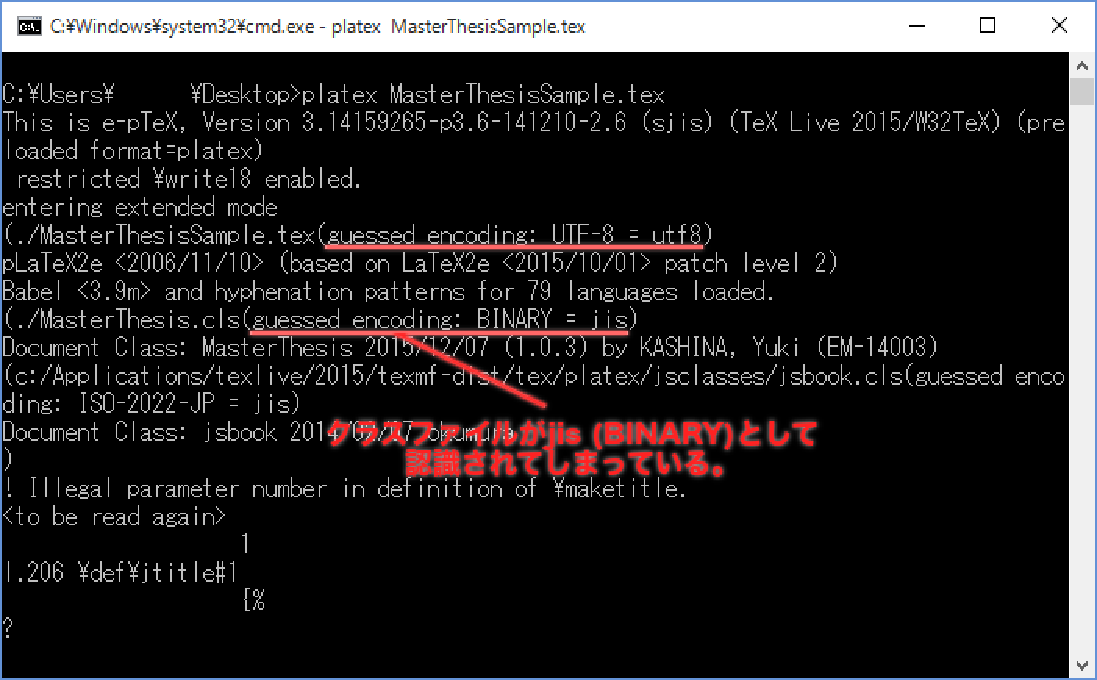
\includegraphics[width=0.9\textwidth]{1.pdf}
	%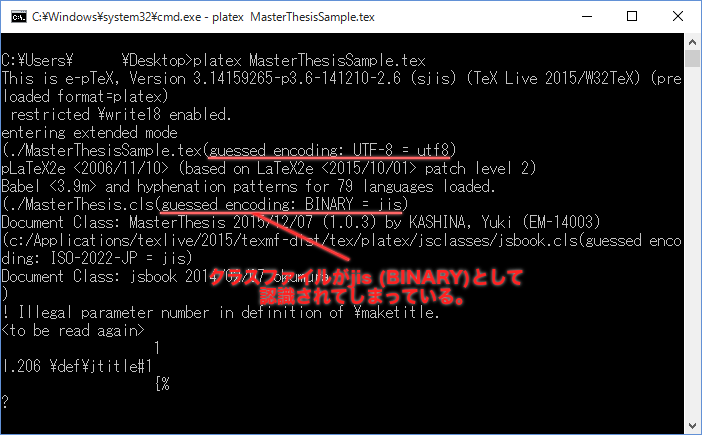
\includegraphics[width=0.9\textwidth]{1.png}
	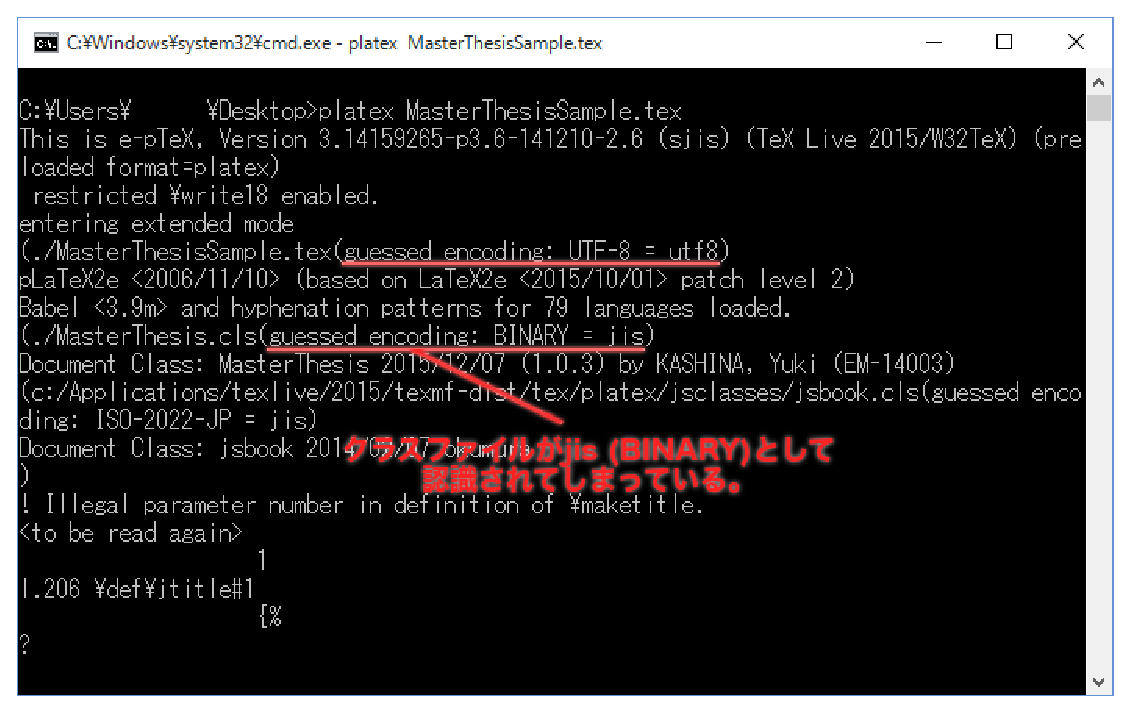
\includegraphics[width=0.9\textwidth]{1.eps}
	\caption{文字コード誤認識によるタイプセットの失敗状況}
	\flabel{ts_failed}
\end{figure}


%%%%%%%%%%%%%%%%%%%%%%%%%%%%%%%%%%%%%%%%%%
% 
\chapter{TeXWorksのpdfpLaTeXでの設定について}
%%%%%%%%%%%%%%%%%%%%%%%%%%%%%%%%


まずは、このファイル(MasterThesisSample.tex)をLaTeXに
かけてPDFファイルが正しく生成されるかテストしてください。

TeXWorksのpdfpLaTeXを実行すると、
以下のようなエラーメッセージが出るかも知れません。

dvipdfmx:warning: Could not locate a virtual/physical font for TFM "hminr-h".

dvipdfmx:warning: >> This font is mapped to a physical font "HiraMinProN-W3.otf".

dvipdfmx:warning: >> Please check if kpathsea library can find this font: HiraMinProN-W3.otf

dvipdfmx:fatal: Cannot proceed without .vf or "physical" font for PDF output...

これはhttp://rexpit.blog29.fc2.com/blog-entry-130.html?sp
に記載されていた以下の手法で解決できました。

(TeXをインストールしたディレクトリ)\textbackslash share\textbackslash texmf-dist\textbackslash fonts\textbackslash map\textbackslash dvipdfmx\textbackslash base にある cid-x.map を開きます。

texインストーラ3のデフォルト設定でインストールした場合には
C:\textbackslash w32tex\textbackslash share\textbackslash texmf-dist\textbackslash fonts\textbackslash map\textbackslash dvipdfmx\textbackslash base\textbackslash cid-x.map
になります。

このファイルの末尾に次の文字列を追記します。

rml         H               Ryumin-Light

rmlv        V               Ryumin-Light

gbm         H               GothicBBB-Medium

gbmv        V               GothicBBB-Medium

hminr-h     H               Ryumin-Light

hminr-v     V               Ryumin-Light

otf-ujmr-h  UniJIS-UTF16-H  Ryumin-Light

otf-ujmr-v  UniJIS-UTF16-V  Ryumin-Light

otf-cjmr-h  Adobe-Japan1-6  Ryumin-Light

otf-cjmr-v  Identity-V      Ryumin-Light

hgothr-h    H               GothicBBB-Medium

hgothr-v    V               GothicBBB-Medium

otf-ujgr-h  UniJIS-UTF16-H  GothicBBB-Medium

otf-ujgr-v  UniJIS-UTF16-V  GothicBBB-Medium

otf-cjgr-h  Adobe-Japan1-6  GothicBBB-Medium

otf-cjgr-v  Identity-V      GothicBBB-Medium


以上です。\footnote{この章のみ、真鍋義文執筆}

%上記のディレクトリパスを、コピーが容易なように
%下に書いておきます。

% C:\w32tex\share\texmf-dist\fonts\map\dvipdfmx\base にある cid-x.map
%


%%%%%%%%%%%%%%%%%%%%%%%%%%%%%%%%%%%%%%%%%%
% 
\chapter{書誌情報の定義と各種設定}
%%%%%%%%%%%%%%%%%%%%%%%%%%%%%%%%%%%%%%%%%%
本章では,標題紙の生成に必要な書誌情報や,その他グローバルな設定の変更方法について説明します。



%%%%%%%%%%%%%%%%%%%%%%%%%%%%%%%%%%%%%%%%%%
% 
\section{書誌情報の定義}
%%%%%%%%%%%%%%%%%%%%%%%%%%%%%%%%%%%%%%%%%%
本節では,標題紙の生成に必要な書式情報を設定するコマンドについて概説します。

\subsection{和文タイトル}
\texcmd{jtitle}コマンドを使います。

\texcmd{newline} で改行できます。コマンドやダブルクォート(\`{}\`{},\'{}\'{})は\{\}によってグルーピングし,\{\`{}\`{}\},\{\'{}\'{}\}のように入力してください。数式では\texcmd{mbox}\{\}によるグルーピングが推奨されます。

\subsection{英文タイトル}
\texcmd{etitle}コマンドを使います。

\texcmd{newline} で改行できます。コマンドやダブルクォート(\`{}\`{},\'{}\'{})は\{\}によってグルーピングし,\{\`{}\`{}\},\{\'{}\'{}\}のように入力してください。数式では\texcmd{mbox}\{\}によるグルーピングが推奨されます。

\subsection{所属専攻}
\texcmd{affiliate}コマンドを使います。記入に際し,``工学研究科''は不要です。

\subsection{氏名}
\texcmd{author}コマンドを使用します。苗字と名前の間に空白スペースを挿入します。また,ルビを振るため\texcmd{ruby}コマンドを使用して,下記のように氏名を記載します。
\[
\mathrm{\backslash{}ruby\{苗字\}\{みょう|じ\}{}_\sqcup\backslash{}ruby\{名前\}\{な|まえ\}}
\]
例文中の${}_\sqcup$は半角スペースを表しています。



\subsection{指導教官名およびその役職}
\texcmd{supervisor}コマンドを使用します。第一引数に指導教官名,第二引数に役職を渡します。指導教官名は,苗字と名前の間に空白スペースを挿入してください。


\subsection{修了年月}
\texcmd{ptdate}コマンドを使用します。第一引数に西暦の修了年,第二引数に修了月を記載します。全角での記入を推奨します。



%%%%%%%%%%%%%%%%%%%%%%%%%%%%%%%%%%%%%%%%%%
% 
\section{各種設定}
%%%%%%%%%%%%%%%%%%%%%%%%%%%%%%%%%%%%%%%%%%
本節では,各種設定を行うためのコマンドについて概説します。

\subsection{前文のタイトル}
\texcmd{abstractname}コマンドで前文のタイトルを設定可能です。デフォルトでは,和文で「要旨」,英文で``Abstract''となっています。

\subsection{目次の有効化}
\texcmd{toctrue}コマンドを使用すると,目次を有効にします。コメントアウトすることで目次の出力を止めることができます。

\subsection{図目次の有効化}
\texcmd{loftrue}コマンドを使用すると,図目次を有効にします。コメントアウトすることで図目次の出力を止めることができます。


\subsection{表目次の有効化}
\texcmd{lottrue}コマンドを使用すると,表目次を有効にします。コメントアウトすることで表目次の出力を止めることができます。

\subsection{索引の有効化}
\texcmd{makeindex}コマンドを使用すると,索引を有効にします。

\subsection{研究室内部資料の有効化}
\texcmd{domestictrue}コマンドを使用すると,付録の研究室内部資料の章を有効にします。

\subsection{fleqnオプション}
本オプションを有効にすると,数式が左寄せになります。デフォルトは中央寄せです。プリアンプルのドキュメントクラス指定時に,オプションとしてfleqnを渡してください。

\subsection{メインフォントサイズの変更}
プリアンブルのフォントサイズ設定の箇所において,本文と記載のある箇所で\texcmd{mainfontsize}マクロを再定義してください。前文,本文のフォントサイズが変わります。

\subsection{英文タイトルのフォントサイズの変更}
プリアンブルのフォントサイズ設定の箇所において,英文タイトルと記載のある箇所で\texcmd{etitlefontsize}マクロを再定義してください。英文タイトルのフォントサイズが変わります。

\subsection{キャプションのフォントサイズの変更}
プリアンブルのフォントサイズ設定の箇所において,キャプションと記載のある箇所で\texcmd{captionfontsize}マクロを再定義してください。キャプションのフォントサイズが変わります。



%%%%%%%%%%%%%%%%%%%%%%%%%%%%%%%%%%%%%%%%%%
% クラスファイルの使用法
\chapter{クラスファイルの使用法}
%%%%%%%%%%%%%%%%%%%%%%%%%%%%%%%%%%%%%%%%%%
本章では,クラスファイルで定義したコマンド等について概説します。



%%%%%%%%%%%%%%%%%%%%%%%%%%%%%%%%%%%%%%%%%%
%
\section{英語対応キャプション}
%%%%%%%%%%%%%%%%%%%%%%%%%%%%%%%%%%%%%%%%%%
従来の\texcmd{caption}コマンドにオプション引数を設け,英文キャプションをつけられるようにしました。オプションをつけなければ,従来通りの\texcmd{caption}コマンドの動作をします。

なお,本修正に伴い,algorithmパッケージなど一部パッケージと競合する場合がありますが,\texcmd{newcaption}や\texcmd{kcaption}の使用により競合(上書き)を回避できるように対策済みです。これらを使用しても競合を回避できないパッケージを使用する場合は,クラスファイルの該当箇所(「キャプションの再定義」の箇所)を削除するなどのクラスファイル修正を行ってください。



%%%%%%%%%%%%%%%%%%%%%%%%%%%%%%%%%%%%%%%%%%
%
\subsection{図キャプションのテスト}
%%%%%%%%%%%%%%%%%%%%%%%%%%%%%%%%%%%%%%%%%%
図のキャプションのテストを行います。\fref{nooption}では\texcmd{caption\{英文キャプションなし\}},\fref{option}では\texcmd{caption[Test of the figure]\{英文キャプションあり\}}として出力しています。
\begin{figure}[h]
	\centering
	\begin{minipage}{.35\textwidth}
		\centering
		\fbox{\rule[0pt]{32pt}{40pt}}
		\caption{英文キャプションなし}
		\flabel{nooption}
	\end{minipage}
	%
	\hfil
	%
	\begin{minipage}{.35\textwidth}
		\centering
		\fbox{\rule[0pt]{32pt}{40pt}}
		\caption[Test of the figure]{英文キャプションあり}
		\flabel{option}
	\end{minipage}
	%
	\commentary{\fref{nooption}では,\texcmd{caption}コマンドのオプションに英文キャプションを渡していないが,\fref{option}では英文キャプションを渡している。このように,本クラスファイルの\texcmd{caption}修正では,同一コマンドで英文キャプションの有無を選択可能な一種のポリモフィズムを実現している。}
\end{figure}
%



%%%%%%%%%%%%%%%%%%%%%%%%%%%%%%%%%%%%%%%%%%
%
\subsection{表キャプションのテスト}
%%%%%%%%%%%%%%%%%%%%%%%%%%%%%%%%%%%%%%%%%%
表のキャプションのテストを行います。\tref{magic1}では\texcmd{kcaption},\tref{magic2}では\texcmd{newcaption}コマンドを使用しています。これらのコマンドは\texcmd{caption}のエイリアスで,algorithmパッケージなど\texcmd{caption}の定義を上書きするパッケージと同時に使用するために定義されています。

\begin{table}[h]
	\centering
	\begin{minipage}{.42\textwidth}
		\centering
		\kcaption[Caption by \texcmd{kcaption}.]{\texcmd{kcaption}によるキャプション}
		\tlabel{magic1}
		\begin{tabular}{l|r}\Hline
			constant & approximate\\ \hline
			$\pi$ & 3.14159265359...\\
			$e$ & 2.71828182846...\\
			$\log_{10}2$ & 0.30102999566...\\ \hline
		\end{tabular}
	\end{minipage}
	%
	\hfil
	%
	\begin{minipage}{.48\textwidth}
	\centering
		\newcaption[Caption by \texcmd{newcaption}.]{\texcmd{newcaption}によるキャプション}
		\tlabel{magic2}
		\begin{tabular}{l|r}\Hline
			constant & approximate\\ \hline
			$\pi$ & 3.14159265359...\\
			$e$ & 2.71828182846...\\
			$\log_{10}2$ & 0.30102999566...\\ \hline
		\end{tabular}
	\end{minipage}
\end{table}



%%%%%%%%%%%%%%%%%%%%%%%%%%%%%%%%%%%%%%%%%%
%
\subsection{外部ファイルからの表の読み込み}
%%%%%%%%%%%%%%%%%%%%%%%%%%%%%%%%%%%%%%%%%%
本クラスファイルには,外部ファイルからの表読み込みを支援するマクロ(\texcmd{includetable})を作成し,組み込んであります。本マクロは,引数として受け取ったファイルを表として読み込み,ラベルを\texcmd{tlabel}により自動定義します。この機能により,ユーザはラベル付けを明示的に行う必要がなくなり,\texcmd{tref}により図番号を簡単に参照することができます。\tref{includetable_test}は外部ファイル(\texttt{./table/includetable\_test.tbl})から読み込んだ表の例です。
%
\begin{table}[bt]
	\centering
	\newcaption[Test for \texcmd{includetable}.]{\texcmd{includetable}による表の読み込みテスト}
	\includetable{includetable_test}
\end{table}
%
\tref{includetable_test}の読み込みコマンドは
\begin{center}\begin{verbatim}\begin{table}[bt]
  \centering
  \newcaption[Test for \texcmd{includetable}.]%
    {\texcmd{includetable}による表の読み込みテスト}
  \includetable{includetable_test}
\end{table}\end{verbatim}\end{center}
です。前述の通り,本マクロはファイル名をラベルとして自動定義します。table環境内で明示的にラベルを定義していないにもかかわらず,\texcmd{tref}により表番号を参照できていることに注目してください(ソースコード参照)。また,プリアンブルで表のルートパスを\texcmd{tablepath}により\texttt{table/}に指定しているため,パスの指定も\texttt{includetable\_test}と簡単化されています(拡張子は\texttt{*.tbl}を期待して自動補完)。



%%%%%%%%%%%%%%%%%%%%%%%%%%%%%%%%%%%%%%%%%%
%
\section{図表と数式の参照}
%%%%%%%%%%%%%%%%%%%%%%%%%%%%%%%%%%%%%%%%%%
ラベルづけ(\texcmd{label})と参照(\texcmd{ref})を簡潔にするため,以下のコマンドを定義しています。
\begin{description}
	\item[\texcmd{flabel},\texcmd{fref}] \dotfill 図のラベルづけと参照
	\item[\texcmd{tlabel},\texcmd{tref}] \dotfill 表のラベルづけと参照
	\item[\texcmd{elabel},\texcmd{eref}] \dotfill 式のラベルづけと参照
\end{description}



%%%%%%%%%%%%%%%%%%%%%%%%%%%%%%%%%%%%%%%%%%
%
\section{章節の参照}
%%%%%%%%%%%%%%%%%%%%%%%%%%%%%%%%%%%%%%%%%%
章の参照も同様のコマンドが定義されています。ただし,図表や式の参照と異なり,{\color{red}接尾辞がlabelではなくlabであることに注意}してください。
\begin{description}
\item[\texcmd{part{\color{red}lab}},\texcmd{partref}] \dotfill 部のラベルづけと参照
\item[\texcmd{chapter{\color{red}lab}},\texcmd{chapterref}] \dotfill 章のラベルづけと参照
\item[\texcmd{section{\color{red}lab}},\texcmd{sectionref}] \dotfill 節のラベルづけと参照
\item[\texcmd{subsection{\color{red}lab}},\texcmd{subsectionref}] \dotfill 項のラベルづけと参照
\end{description}



%%%%%%%%%%%%%%%%%%%%%%%%%%%%%%%%%%%%%%%%%%
% まとめ
\chapter{まとめ}
%%%%%%%%%%%%%%%%%%%%%%%%%%%%%%%%%%%%%%%%%%
本ドキュメントでは工学院大学大学院工学研究科用修士学位請求論文\LaTeX テンプレートの使い方を概説しました。

拙筆ながらも,本クラスファイル・テンプレートが情報学専攻\LaTeX 使用者の修論執筆の一助となれば幸いです。また,有志の修士・先生方による改良を歓迎いたします。



%%%%%%%%%%%%%%%%%%%%%%%%%%%%%%%%%%%%%%%%%%
% 謝辞
\acknowledge{謝辞}
%%%%%%%%%%%%%%%%%%%%%%%%%%%%%%%%%%%%%%%%%%
``24階修論グループ''の熊谷洋佑さん(先進ソフトウェア研究室),峯祥平さん(インタラクティブメディア研究室),坂田直人さん(数理音響学研究室)には,クラスファイルの試用や機能の提案をはじめとする多くの協力と助言をしていただきました。ここに感謝いたします。

ベースクラスファイルとしてjsbook,均等割り付けの実装に名古屋大学大学院多元数理科学研究科~久保仁さんの\texcmd{fitwidth}マクロ\cite{fitwidth}を使用させていただきました。

論文標題の下線で用いられている,ページ幅の下線を引く実装(\texcmd{ulfill})において,udline.sty ver2.52(2005/01/28)\cite{udline}を参考にさせていただきました。



%%%%%%%%%%%%%%%%%%%%%%%%%%%%%%%%%%%%%%%%%%
% 参考文献
\references{参考文献}%タイトル変更可能
%%%%%%%%%%%%%%%%%%%%%%%%%%%%%%%%%%%%%%%%%%
%\bibliographystyle{junsrt}
%\bibliography{}
%bibtexを使う方は,以下をコメントアウトし,上記を有効にする。スタイルは適宜変更のこと。
\begin{thebibliography}{99}
	\bibitem{udline} http://homepage2.nifty.com/domae/tex/udline.html
	\bibitem{fitwidth} http://www.math.nagoya-u.ac.jp/\textasciitilde{}kubo/ja/latex/tips-003.html
	\bibitem{c1} (雑誌の場合;雑誌とは論文誌等のこと)著者名, ``標題, '' 雑誌名, 巻, 号, pp.A--B, Month, 年.
	\bibitem{c2} (著書,編書の場合)著者名, 書名, 編者名, 発行所, 発行都市名, 発行年.
	\bibitem{c3} (著書の一部を引用する場合)著者名, ``標題, '' 書名, 編者名, 章番号またはpp.A--B, 発行所, 発行都市名, 発行年.
	\bibitem{c4} (国際学会論文集の場合)著者名, ``標題, '' 会議名, no.A, pp.B--C, 都市名, 国名, Month, 年.
	\bibitem{c5} (国内学会,研究会論文集の場合)著者名, ``標題, '' 学会論文集名, vol.A, no.B, pp.C--D, 都市名, 国名, Month, 年.
\end{thebibliography}



%%%%%%%%%%%%%%%%%%%%%%%%%%%%%%%%%%%%%%%%%%%%%%%%%%%%%%
% 発表実績
\publications{本研究に関する発表}
%%%%%%%%%%%%%%%%%%%%%%%%%%%%%%%%%%%%%%%%%%%%%%%%%%%%%%
\begin{thepublication}
%
\publicationtype{論文}
\item \underline{1st Author}, 2nd Author, 3rd Author, Last Author, ``Title,'' Society, Year.
%
\publicationtype{査読付き会議}
\item \underline{1st Author}, 2nd Author, 3rd Author, Last Author, ``Title,'' Conference, Year.
\item 1st Author, \underline{2nd Author}, 3rd Author, Last Author, ``Title,'' Workshop, Year.
%
\publicationtype{研究会}
\item \underline{1st Author}, 2nd Author, 3rd Author, Last Author, ``Title,'' Conference, Year.
%
\publicationtype{全国大会}
\item \underline{1st Author}, 2nd Author, 3rd Author, Last Author, ``Title,'' Conference, Year.
%
\end{thepublication}



%%%%%%%%%%%%%%%%%%%%%%%%%%%%%%%%%%%%%%%%%%
% 付録
\appendix
%%%%%%%%%%%%%%%%%%%%%%%%%%%%%%%%%%%%%%%%%%
\chapter{ソースコード}
お手元のMasterThesis.cls,MasterThesisSample.texをご参照ください。


\chapter{更新履歴}
%
%-----------------------------------
\section*{\ulfill{Version 2.0.x}}
%-----------------------------------
\subsection*{Version 2.0.1 (December 24, 2015, Thursday)}
\begin{itemize}
	\item \texcmd{ulfill}を実装し,既存の標題の下線と差し替え
	\item プリアンブルでのみ使用可能であるべきコマンドに対しプリアンブルでの使用を強制
	\item デフォルトフォントサイズを変更(本文:12pt,英語タイトル14pt,キャプション11pt)
	\item ドキュメント整理
	\item Merry X'mas!!
\end{itemize}
%
%-----------------------------------
\section*{\ulfill{Version 1.0.x}}
%-----------------------------------
%%%
\subsection*{Version 1.0.8 (December 24, 2015, Thursday)}
\begin{itemize}
	\item タイトルの下線の処理を修正
\end{itemize}

%%%
\subsection*{Version 1.0.7 (December 24, 2015, Thursday)}
\begin{itemize}
	\item 発表実績の章を執筆するためのthepublication環境を作成
	\item thepublication環境で使用する\texcmd{publicationtype}コマンドを定義
\end{itemize}

%%%
\subsection*{Version 1.0.6 (December 21, 2015, Monday)}
\begin{itemize}
	\item キャプションのサイズを変更可能にし,デフォルトを12ptに変更
	\item 英語タイトルのフォントサイズを変更可能にし,デフォルトを20ptから14ptに変更
	\item history.txtを付録に統合
\end{itemize}

%%%
\subsection*{Version 1.0.5 (December 20, 2015, Friday)}
\begin{itemize}
	\item 英語Abstractのインデントをハーフインチ(.5in)に変更
	\item 英語Abstractのファーストインデントのみ字下げしないようにした
\end{itemize}

%%%
\subsection*{Version 1.0.4 (December 18, 2015, Friday)}
\begin{itemize}
	\item 関連発表用のコマンド(\texcmd{publications})を作成
	\item 参考文献の章タイトルを任意に設定可能な仕様に変更(\texcmd{references})
	\item \texcmd{graphicspath\{\{fig/\}\}}を追加
	\item 研究室内部資料用のコマンド(\texcmd{domestictrue})を作成
	\item 表の最上部罫線用コマンド(\texcmd{Hline})を作成(太罫線)
\end{itemize}

%%%
\subsection*{Version 1.0.3 (December 7, 2015, Monday)}
\begin{itemize}
	\item 目次にハイパーリンクを追加
	\item fleqnオプションの追加
	\item デフォルトを中央寄せに
\end{itemize}

%%%
\subsection*{Version 1.0.2 (December 4, 2015, Friday)}
\begin{itemize}
	\item 英語キャプションを追加
	\item その他修正
\end{itemize}

%%%
\subsection*{Version 1.0.1 (November 28, 2015, Saturday)}
初版



%%%%%%%%%%%%%%%%%%%%%%%%%%%%%%%%%%%%%%%%%%%%%%%%%%%%%%
% 研究室内部用の資料
\begin{domestic}
%%%%%%%%%%%%%%%%%%%%%%%%%%%%%%%%%%%%%%%%%%%%%%%%%%%%%%
\chapter{ファイルの場所}
本論文のファイル一式は研究室共有の...に保存してあります。実験プロジェクト等は研究室共有の...に保存してあります。


\chapter{引き継ぎ資料}
実験プロジェクトの使用法や,その他端書きは研究室共有の...に保存してあります。



%%%%%%%%%%%%%%%%%%%%%%%%%%%%%%%%%%%%%%%%%%
% 文書の終わり
%%%%%%%%%%%%%%%%%%%%%%%%%%%%%%%%%%%%%%%%%%
\end{domestic}
\eof%End-Of-File
%%%\end{document}は不要です